%\documentclass[10pt,times,twocolumn]{paper}
\documentclass[english,aps,prd,nofootinbib,twocolumn]{revtex4-1}
%\documentclass[english,aps,prd,nofootinbib]{revtex4-1}
%\documentclass[twocolumn,english,aps,prd,nofootinbib]{revtex4-1}
\usepackage{CJK}

%\usepackage{tikz}
\usepackage{amsfonts}
\usepackage{amsmath}
\usepackage{hyperref}
\usepackage{amssymb}
\usepackage{cleveref}
\usepackage{cancel}
\usepackage{xfrac}
\usepackage{xcolor}
\usepackage{relsize}%\mathlarger command 
%\usetikzlibrary{arrows,decorations.markings}
\usepackage[bottom]{footmisc}

%\usepackage{newtxtext}
%\usepackage{multicol}
%\usepackage{comment}
\usepackage{tikz}
\usepackage{tikz-feynman}
\usetikzlibrary{calc,arrows,decorations.markings,snakes,shapes}
\usepackage{pgfplots}
\pgfplotsset{compat=1.3}
\usetikzlibrary{3d,calc}

\newcommand{\tstar}[5]{% inner radius, outer radius, tips, rot angle, options
\pgfmathsetmacro{\starangle}{360/#3}
\draw[#5] (#4:#1)
\foreach \x in {1,...,#3}
{ -- (#4+\x*\starangle-\starangle/2:#2) -- (#4+\x*\starangle:#1)
}
-- cycle;
}

\newcommand{\ngram}[4]{% outer radius, tips, rot angle, options
\pgfmathsetmacro{\starangle}{360/#2}
\pgfmathsetmacro{\innerradius}{#1*sin(90-\starangle)/sin(90+\starangle/2)}
\tstar{\innerradius}{#1}{#2}{#3}{#4}
}

%\usepackage{subfigure}
%\usepackage{subcaption}
%\captionsetup[subfigure]{labelformat=brace}

%\usetikzlibrary{tikzmark,fit}

\usepackage{units}

%%%%%%%%%%%%%%%%%%%%%%%%%%%%%%%%%%%%%%%%%%%%%%%%%%%%%%%%%%

\newcommand{\sfms}[1]{\textbf{\textcolor{blue}{(#1 --Seb)}}}
\newcommand{\inti}[1]{\textbf{\textcolor{green}{(#1 --El Jefe)}}}

\renewcommand{\textfraction}{0.10}
\renewcommand{\topfraction}{0.90}
\renewcommand{\bottomfraction}{0.90}
\renewcommand{\floatpagefraction}{0.65}

\usepackage{xspace}



%%%%%%%%%%%%%%%%%%%%%%%%%%%%%%%%%%%%%%%%%%%%%%%%%%%%%%%%%%

\usepackage{color}
\usepackage{graphicx}
\usepackage[space]{grffile}
%\usepackage{indentfirst}
\usepackage{verbatim}
\usepackage{amsmath}
\usepackage{amssymb}
\usepackage{wasysym}
\usepackage[caption=false]{subfig}
\usepackage{url}
\usepackage{bbold}
\usepackage{slashed}
\usepackage{epstopdf}
\usepackage{braket}
\usepackage{float}

%\usepackage{biblatex}

\newcommand{\aaps}{{Astron.~Astrophys.~Supp.}}
\newcommand{\physrep}{{Physics~Reports}}
\newcommand{\araa}{{Annu.~Rev.~Astron.~Astrophys.}}
\newcommand{\aap}{{Astron.~Astrophys.}}
\newcommand{\apjl}{{Astrophys.~J.~Lett.}}
\newcommand{\apjs}{{Astrophys.~J.~Supp.}}
\newcommand{\aj}{{Astron.~J.}}
%\newcommand{\apj}{The Astrophysics Journal}
\newcommand{\mnras}{{Mon.~Not.~R.~Astron.~Soc.}}
\newcommand{\aapr}{{Astronomy and Astrophysics Reviews}}

\DeclareRobustCommand{\Sec}[1]{Sec.~\ref{#1}}
\DeclareRobustCommand{\Secs}[2]{Secs.~\ref{#1} and \ref{#2}}
\DeclareRobustCommand{\App}[1]{App.~\ref{#1}}
\DeclareRobustCommand{\Tab}[1]{Table~\ref{#1}}
\DeclareRobustCommand{\Tabs}[2]{Tables~\ref{#1} and \ref{#2}}
\DeclareRobustCommand{\Fig}[1]{Fig.~\ref{#1}}
\DeclareRobustCommand{\Figs}[2]{Figs.~\ref{#1} and \ref{#2}}
\DeclareRobustCommand{\Eq}[1]{Eq.~(\ref{#1})}
\DeclareRobustCommand{\Eqs}[2]{Eqs.~(\ref{#1}) and (\ref{#2})}
\DeclareRobustCommand{\Ref}[1]{Ref.~\cite{#1}}
\DeclareRobustCommand{\Refs}[1]{Refs.~\cite{#1}}
\DeclareMathAlphabet\mathbfcal{OMS}{cmsy}{b}{n}

\newcommand{\boundellipse}[3]% center, xdim, ydim
{[black,fill=blue!30] (#1) ellipse (#2 and #3)
}
\newcommand{\boundellipseW}[3]% center, xdim, ydim
{[white,fill=white] (#1) ellipse (#2 and #3)
}
\newcommand*{\Scale}[2][4]{\scalebox{#1}{$#2$}}%
\newcommand*{\Resize}[2]{\resizebox{#1}{!}{$#2$}}%
\DeclareMathOperator*{\Motimes}{\text{\raisebox{0.25ex}{\scalebox{0.8}{$\bigotimes$}}}}
%\usepackage{mathabx,graphicx}
\def\Circlearrowleft{\ensuremath{%
  \rotatebox[origin=c]{180}{$\circlearrowleft$}}}
\def\Circlearrowright{\ensuremath{%
  \rotatebox[origin=c]{180}{$\circlearrowright$}}}
\def\CircleArrowleft{\ensuremath{%
  \reflectbox{\rotatebox[origin=c]{180}{$\circlearrowleft$}}}}
\def\CircleArrowright{\ensuremath{%
  \reflectbox{\rotatebox[origin=c]{180}{$\circlearrowright$}}}}



\begin{document}

\title{Multilayer graphene}

%\author{Sebastian Mantilla$^{1}$}
%\email{mantilla@pks.mpg.de}
%\author{Inti Sodemann$^{1}$}
%\email{sodemann@pks.mpg.de}


%\affiliation{$^1$Department of Physics, Princeton University, Princeton, NJ 08544}

%\affiliation{$^1$Max-Planck Institute for the Physics of Complex Systems, D-01187 Dresden, Germany}

%\date{\today}


%\maketitle	

\section*{Multilayer graphene}

%\tableofcontents



%\begin{abstract}
%We develop a bosonization formalism that captures non-perturbatively the interaction effects on the $\mathbf{Q}=0$ continuum of excitations of nodal fermions above one dimension. Our approach is a natural extension of the classic bosonization scheme for higher dimensional Fermi surfaces 
%~\cite{luther1979tomonaga, haldane2005luttinger, houghton1993bosonization, neto1994bosonization} 
%to include the $\mathbf{Q}=0$ neutral excitations that would be absent in a single-band system. The problem is reduced to solving a boson bilinear Hamiltonian. We establish a rigorous microscopic footing for this approach by showing that the solution of such boson bilinear Hamiltonian is exactly equivalent to performing the infinite sum of Feynman diagrams associated with the Kadanoff-Baym particle-hole propagator that arises from the self-consistent Hartree-Fock approximation to the single particle Green's function. We apply this machinery to compute the interaction corrections to the optical conductivity of 2D Dirac Fermions with Coulomb interactions reproducing the results of perturbative renormalization group at weak coupling and extending them to the strong coupling regime. 
%\end{abstract}


\section{Scales of the Hamiltonian}
We set $\hbar = 1$ throughout all the text. The UV cutoff $\mathcal{K}$ of the system, fixed by the lattice parameter $2\pi/\mathcal{K}$, provides us a natural scale to measure the momenta, such that any momentum index $\mathbf{k}$ is normalized by $\mathcal{K}$. In this way, we get the kinetic non-interacting Hamiltonian
\begin{equation}
\label{eq:Main-Ham}
\begin{split}
&H_{\mathrm{kin}} = 
E_{\mathrm{UV} }\sum_{\mathbf{k }\sigma\sigma'}
\left(\frac{|\mathbf{k}|}{\mathcal{K}}\right)^{m}
\psi_{\mathbf{k },\sigma}^{\textcolor{black}{\dagger}}
\left( \hat{\mathbf{n}}_{m} \cdot 
\boldsymbol{\sigma}_{\sigma\sigma'} \right)
\psi_{\mathbf{k },\sigma'}^{\textcolor{white}{\dagger}}
,
\end{split}
\end{equation}
where $[\hat{\mathbf{n}}_{m}]= 
\begin{pmatrix}
\cos(m\phi_{m})	&	\!\!\sin(m\phi_{m})
\end{pmatrix}$ and $E_{\mathrm{UV} }$ is the numerical value of the kinetic term evaluated at $\mathcal{K}$, and whose shape depends on $m$:
\begin{itemize}
\item $m=1$: $E_{\mathrm{UV} } = v\mathcal{K}$, where $v$ is the Fermi velocity of the Dirac fermions.
\item $m=2$: $E_{\mathrm{UV} } = \mathcal{K}^{2}/2m_{e}$, where $m_{e}$ is the effective mass of the electron. 
\end{itemize}
The potential is given by
\begin{equation}
V_{\mathbf{r}} = 
V_{0}e^{-r^{2}/2a^{2}}
\end{equation}
with $V_{0}$ the intensity of the Gaussian potential and $a$ the spreading in the real space. Its Fourier transform is
\begin{eqnarray*}
\nonumber	
V_{\mathbf{k}} = 2\pi a^{2}V_{0}
e^{-\tfrac{a^{2}k^{2}}{2}}\!
= \frac{E_{\mathrm{UV}}}{\mathcal{K}^{2}} 
\left[ \frac{2\pi (a\mathcal{K})^{2}V_{0}}{E_{\mathrm{UV}}}
e^{-\tfrac{(a{\mathcal{K}})^{2}}{2}
\left( \tfrac{k}{\mathcal{K}} \right)^{2}}
\right],	
\end{eqnarray*}
\vspace{-.5cm}
\begin{equation}
\label{eq:Fourier-Potential}
V_{\mathbf{k}} = \frac{E_{\mathrm{UV}}}{\mathcal{K}^{2}} 
\left( g_{0} 
e^{-\tfrac{a_{\mathcal{K}}^{2}}{2}
\left( \tfrac{k}{\mathcal{K}} \right)^{2}}
\right),	
\end{equation}
where $k=|\mathbf{k}|$. It is assumed that $a>2\pi/\mathcal{K}$, i.e., the spreading of the Gaussian should be larger than the lattice parameter $2\pi/\mathcal{K}$. The additional two nondimensional parameters are:
\begin{itemize}
\item $a_{\mathcal{K}}=a\mathcal{K}$: Determines how concentrated is the potential in the reciprocal space. It is constrained to be larger than one.
\item $g_{\mathcal{K}}=2\pi a_{\mathcal{K}}^{2}V_{0}/E_{\mathrm{UV}}$: Relates the intensity of the Gaussian potential in the reciprocal space with $E_{\mathrm{UV}}$, the kinetic energy at the UV cutoff.
\end{itemize}
Lastly, the interaction Hamiltonian can be expressed as
\begin{eqnarray}
&H&\!_{\mathrm{int}} =
\frac{1}{2A}
%\sum_{\genfrac{ }{ }{0pt}{3}{\mathbf{k },\mathbf{k'}}{\mathbf{q }\neq 0} } 
\sum_{\mathbf{k }\mathbf{k'}}
\sum_{\sigma \sigma'} 
V_{\mathbf{q}}
\psi_{\mathbf{k'+q,\sigma'}}^{\textcolor{black}{\dagger}}
\psi_{\mathbf{k -q,\sigma }}^{\textcolor{black}{\dagger}}
\psi_{\mathbf{k   ,\sigma }}^{\textcolor{white}{\dagger}}
\psi_{\mathbf{k'  ,\sigma'}}^{\textcolor{white}{\dagger}} \\
 &=& \nonumber \frac{E_{\mathrm{UV}}}{2A\mathcal{K}^{2}}
\sum_{\mathbf{k }\mathbf{k'}}
\sum_{\sigma \sigma'} 
g_{\mathcal{K}}
e^{-\tfrac{a_{\mathcal{K}}^{2}}{2}\left( \tfrac{k}{\mathcal{K}} \right)^{2}}
\!\! 
\psi_{\mathbf{k'+q,\sigma'}}^{\textcolor{black}{\dagger}}
\psi_{\mathbf{k -q,\sigma }}^{\textcolor{black}{\dagger}}
\psi_{\mathbf{k   ,\sigma }}^{\textcolor{white}{\dagger}}
\psi_{\mathbf{k'  ,\sigma'}}^{\textcolor{white}{\dagger}}.
\end{eqnarray}
where $A$ is the total area of the system.

\section{Restricted Hilbert space for $\mathbf{Q}=0$ excitons and pseudospin basis}
\begin{figure}
\centering
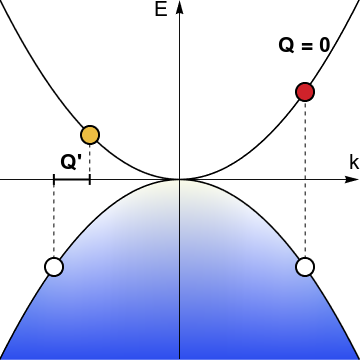
\includegraphics[scale=0.45]{ParabolicVertical.png}
\caption{$\mathbf{Q}=0$ and $\mathbf{Q}\neq 0$ excitations on the parabolic bands.}
\label{fig:Q=0-excitons}
\end{figure}

The optical relevant excitations of the system correspond to the $\mathbf{Q}=0$ excitons, as shown in FIG. \ref{fig:Q=0-excitons}. These ones do not modify the momentum label of the electron when it jumps from the valence to the conduction band, and consequently, any interaction between a pair excitons at momenta $\mathbf{k}_{1}$ and $\mathbf{k}_{2}$ should only interchange their momentum labels. In other words, by having into account only $\mathbf{Q}=0$ excitations, the Hilbert space of the system results restricted onto the singly-occupied sites in the momentum lattice. A good operator to describe the singly-occupied constrain is
\begin{equation}
\label{eq:SU(2)-spin-operator}
s^{\mu}_{\mathbf{k }} = \sum_{\sigma \sigma'} 
\psi_{\mathbf{k ,\sigma }}^{\textcolor{black}{\dagger}}
\sigma^{\mu }_{\sigma \sigma'}
\psi_{\mathbf{k ,\sigma'}}^{\textcolor{white}{\dagger}}.
\end{equation}
where $\sigma^{\mu }_{\sigma  ,\sigma '}$ is the component $\sigma \sigma '$ of the matrix $\sigma^{\mu }$, given by the generators ot the SU(2) Lie algebra, i.e., the Pauli matrices and the identity
\begin{equation}
\begin{matrix}
\sigma^{0}_{\textcolor{white}{,}} = 
\begin{pmatrix}
1	&	0	\\	0	&	1
\end{pmatrix}	&	,	&	
\sigma^{1}_{\textcolor{white}{,}} = 
\begin{pmatrix}
0	&	1	\\	1	&	0
\end{pmatrix}	&	, \\
\sigma^{2}_{\textcolor{white}{,}} = 
\begin{pmatrix}
0	&	-i	\\	i	&	0
\end{pmatrix}	&	,	&	
\sigma^{3}_{\textcolor{white}{,}} = 
\begin{pmatrix}
1	&	0	\\	0	&	-1
\end{pmatrix}	&	,
\end{matrix}
\end{equation}
The matrix $\sigma^{0}$ is useful to express the singly-occupied condition as the constrain
\begin{equation}
\begin{split}
s^{0}_{\mathbf{k }} &= \sum_{\sigma \sigma'} 
\psi_{\mathbf{k ,\sigma }}^{\textcolor{black}{\dagger}}
\sigma^{0}_{\sigma \sigma'}
\psi_{\mathbf{k ,\sigma'}}^{\textcolor{white}{\dagger}} =
\sum_{\sigma \sigma'} 
\psi_{\mathbf{k ,\sigma }}^{\textcolor{black}{\dagger}}
\delta_{\sigma \sigma'}
\psi_{\mathbf{k ,\sigma'}}^{\textcolor{white}{\dagger}} \\ &=
\sum_{\sigma \sigma'} 
\psi_{\mathbf{k ,\sigma }}^{\textcolor{black}{\dagger}}
\psi_{\mathbf{k ,\sigma }}^{\textcolor{white}{\dagger}} =
\sum_{\sigma } 
n_{\mathbf{k ,\sigma }} = 
1.
\end{split}
\end{equation}.

The following steps show how the four-fermion term in the interacion Hamiltonian can be expressed under the singly-occupied constrain. The completeness relation of the Pauli matrices
\begin{equation}
\sum_{\mu=0}^{3} 
\sigma^{\mu }_{\sigma \sigma'}\sigma^{\mu }_{\tau \tau'} =  
2 \delta_{\sigma \tau'} \delta_{\sigma'\tau },
\end{equation}
and the trace of Pauli matrices bilinears 
\begin{equation}
\mathrm{tr}\left( \sigma^{\mu }\sigma^{\mu'} \right) = 
\sum_{\tau ,\tau'}
\sigma^{\mu }_{\tau \tau'}\sigma^{\mu'}_{\tau'\tau } = 
2 \delta^{\mu \mu'},
\end{equation}
are useful to find the inverse relation between fermion bilinears and Pauli matrices
\begin{equation}
\begin{split}
\sum_{\mu=0}^{3} 
\sigma^{\mu }_{\tau \tau'}s^{\mu}_{\mathbf{k }} &= 
\sum_{\mu=0}^{3} \sum_{\sigma \sigma'} 
\psi_{\mathbf{k ,\sigma }}^{\textcolor{black}{\dagger}}
\sigma^{\mu }_{\sigma \sigma'}\sigma^{\mu }_{\tau ,\tau'}
\psi_{\mathbf{k ,\sigma'}}^{\textcolor{white}{\dagger}} \\ &= 
2
\sum_{\sigma \sigma'} 
\psi_{\mathbf{k ,\sigma }}^{\textcolor{black}{\dagger}}
\delta_{\sigma \tau'} \delta_{\sigma'\tau }
\psi_{\mathbf{k ,\sigma'}}^{\textcolor{white}{\dagger}} \\ &= 
2
\psi_{\mathbf{k ,\tau'}}^{\textcolor{black}{\dagger}}
\psi_{\mathbf{k ,\tau }}^{\textcolor{white}{\dagger}} .
\end{split}
\end{equation}
In this way, the fermion bilinears can then be expanded in terms of the generators of the Lie algebra of the group $\mathrm{SU}(2)$
\begin{equation}
\label{eq:SU(2)-expansion-of-fermion-bilinears}
\psi_{\mathbf{k ,\tau'}}^{\textcolor{black}{\dagger}}
\psi_{\mathbf{k ,\tau }}^{\textcolor{white}{\dagger}} = 
\frac{1}{2}
\sum_{\mu=0}^{3} 
s^{\mu }_{\mathbf{k }}\sigma^{\mu }_{\tau \tau'},
\end{equation}

The Eq. \eqref{eq:SU(2)-expansion-of-fermion-bilinears}
is then useful to express the four-fermion term of the interaction Hamiltonian after some anticommutations to match fermion operators that share the same momentum label, such as follows
\begin{equation}
\begin{split}
\sum_{\tau ,\tau'}&
\left(\psi_{\mathbf{k ,\tau   }}^{\textcolor{black}{\dagger}}
\psi_{\mathbf{k ,\tau'  }}^{\textcolor{white}{\dagger}}\right)
\left(\psi_{\mathbf{k',\sigma }}^{\textcolor{black}{\dagger}}
\psi_{\mathbf{k',\sigma'}}^{\textcolor{white}{\dagger}}\right)
 = \\ &=
\sum_{\tau ,\tau'}
\left(
\frac{1}{2} 
\sum_{\mu =0}^{3} 
\sigma^{\mu }_{\tau'\tau }s^{\mu }_{\mathbf{k }}
\right)
\left(
\frac{1}{2} 
\sum_{\mu'=0}^{3} 
\sigma^{\mu'}_{\tau \tau'}s^{\mu'}_{\mathbf{k'}}
\right) \\ &=
\frac{1}{4}
\sum_{\mu ,\mu'}
s^{\mu }_{\mathbf{k }}
s^{\mu'}_{\mathbf{k'}}
\sum_{\tau ,\tau'}
\sigma^{\mu }_{\tau'\tau }
\sigma^{\mu'}_{\tau \tau'}
 \\ &=
\frac{1}{4}
\sum_{\mu ,\mu'}
s^{\mu }_{\mathbf{k }}
s^{\mu'}_{\mathbf{k'}}
\mathrm{tr}\left( \sigma^{\mu }\sigma^{\mu'} \right)
\\ &=
\frac{1}{2}
\sum_{\mu ,\mu'}
s^{\mu }_{\mathbf{k }}
s^{\mu'}_{\mathbf{k'}}
\delta^{\mu \mu'}
=
\frac{1}{2}
\sum_{\mu ,\mu'}
s^{\mu }_{\mathbf{k }}
s^{\mu }_{\mathbf{k'}}
=
\frac{
1 + 
\mathbf{s}_{\mathbf{k }}
\cdot
\mathbf{s}_{\mathbf{k'}}
}{2}
\end{split}
\end{equation}

Consequently, the original fermion Hamiltonian projected onto the singly-occupied is expressed as
\begin{equation}
\label{eq:Effective-Heisenberg-Hamiltonian}
\begin{split}
\mathcal{P} H \mathcal{P} &= \\
E_{\mathrm{UV} }&
\sum_{\mathbf{k }} \left(\frac{|\mathbf{k}|}{\mathcal{K}}\right)^{m}
\!\! 
\hat{\mathbf{k}}_{m}\!\! \cdot \mathbf{s}_{\mathbf{k }} - 
\sum_{\mathbf{k}_{1} \neq \mathbf{k}_{2}}
%\overbrace{
\frac{V_{\mathbf{k}_{1}-\mathbf{k}_{2}}}{4A}
\mathbf{s}_{\mathbf{k}_{1}}\!\!
\cdot
\mathbf{s}_{\mathbf{k}_{2}}
,
\end{split}
%}^{Ferromag.\;exchange}
\end{equation}
where the first term represents a $m$-folded spin vortex (see FIG. \ref{fig:Classical-gound-state}) and the second term is an effective ferromagnetic exchange. 

\section{Expansion about the non-interacting ground state}


\subsection{Band basis and interaction matrix}
\label{sect:Supp:Band-basis}

\begin{figure}
\centering
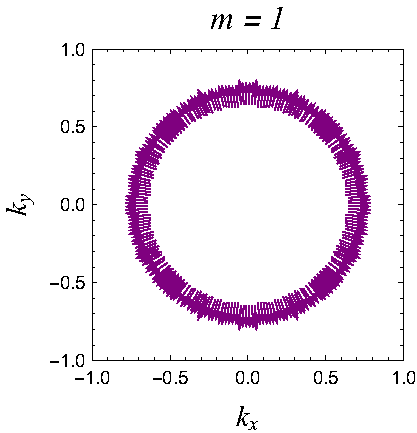
\includegraphics[scale=0.8]{1Layer.pdf}
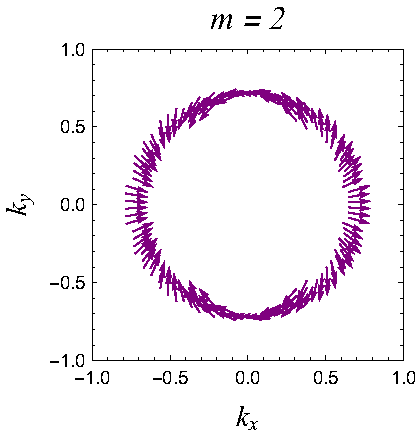
\includegraphics[scale=0.8]{2Layer.pdf}
%\includegraphics[scale=0.8]{3Layer.pdf}
%\includegraphics[scale=0.8]{4Layer.pdf}
%\includegraphics[scale=0.8]{5Layer.pdf}
%\includegraphics[scale=0.8]{6Layer.pdf}
\caption{Polar distribution of the vector $[\hat{\mathbf{n}}_{m}]= 
\begin{pmatrix}
\cos(m\phi_{m})	&	\!\!\sin(m\phi_{m})
\end{pmatrix}$ used to describe the classical ground state of the system.}
\label{fig:Classical-gound-state}
\end{figure}

In this section, we provide details of the derivation of Eqs. \eqref{eq:HP-Hamiltonian} to \eqref{eq:Interacion-matrix} starting from Eq. \eqref{eq:Main-Ham}. We begin describing the transfomation from pseudo-spin basis onto band basis. In the band basis $s=\{+,-\}$ the kinetic term is:
\begin{equation}
\begin{split}
\psi_{\mathbf{k }\sigma }^{\textcolor{black}{\dagger}}&
\left( \hat{\mathbf{k}}_{m} \cdot 
\boldsymbol{\sigma}_{\sigma\sigma'} \right)
\psi_{\mathbf{k }\sigma'}^{\textcolor{white}{\dagger}}
 = 
\\ &= 
    e^{-im\phi}
    \psi_{\mathbf{k\uparrow  }}^{\textcolor{black}{\dagger}}
    \psi_{\mathbf{k\downarrow}}^{\textcolor{white}{\dagger}} + 
    e^{+im\phi}
    \psi_{\mathbf{k\downarrow}}^{\textcolor{black}{\dagger}}
    \psi_{\mathbf{k\uparrow  }}^{\textcolor{white}{\dagger}} 
    .
\end{split}
\end{equation}
Band and pseudospin basis are related by:
\begin{equation}
\begin{split}
	\psi_{\mathbf{k}\sigma} &= 
	\sum_{s}
	\left\langle \sigma | \mathbf{k }s \right\rangle
	\psi_{\mathbf{k} s },	\\
\begin{pmatrix}
    \psi_{\mathbf{k\uparrow  }}	\\
    \psi_{\mathbf{k\downarrow}}	
\end{pmatrix} &= 
\frac{1}{\sqrt{2}}
\begin{pmatrix}
	 e^{- im\phi /2}	& 
	 e^{- im\phi /2}	\\  
	 e^{+ im\phi /2}	&
    -e^{+ im\phi /2}
\end{pmatrix}
\begin{pmatrix}
	\psi_{\mathbf{k+}}	\\
	\psi_{\mathbf{k-}}	
\end{pmatrix}.
\end{split}
\end{equation}
Fermion bilinears transform as
\begin{equation}
\begin{split}
\sum_{\sigma}
\psi_{\mathbf{k}_{1}\sigma}^{\textcolor{black}{\dagger}}
\psi_{\mathbf{k}_{2}\sigma}^{\textcolor{white}{\dagger}}
&= 
\psi_{\mathbf{k}_{1}s_{1} }^{\textcolor{black}{\dagger}}
\sum_{s_{1}s_{2}}\!\!
\left\langle \mathbf{k}_{1}s_{1} | \mathbf{k}_{2}s_{2} \right\rangle \psi_{\mathbf{k}_{1}s_{1} }^{\textcolor{black}{\dagger}}
\psi_{\mathbf{k}_{2}s_{2} }^{\textcolor{white}{\dagger}},
\end{split}
\end{equation}
where
\begin{equation}
\begin{split}
& \left\langle \mathbf{k}_{1}s_{1} | \mathbf{k}_{2}s_{2} \right\rangle =
\begin{pmatrix}
     \cos\sfrac{m\phi_{12}}{2}  &    i\sin\sfrac{m\phi_{12}}{2} \\  
    i\sin\sfrac{m\phi_{12}}{2}  &     \cos\sfrac{m\phi_{12}}{2}
\end{pmatrix},
\end{split}
\end{equation}
where $\phi_i$ is the polar angle of $\mathbf{k}_i$, and  $\phi_{12}=\phi_1-\phi_2$. Therefore, the Hamiltonian in Eq. \eqref{eq:Main-Ham} of the Main text in the band basis is expressed as follows:
\begin{equation}
\begin{split}
&\mathcal{P} H \mathcal{P} = 
\sum_{\mathbf{k }}E^{m}_{\mathbf{k}}
\left( 
\psi_{\mathbf{k}+ }^{\textcolor{black}{\dagger}}
\psi_{\mathbf{k}+ }^{\textcolor{white}{\dagger}} - 
\psi_{\mathbf{k}- }^{\textcolor{black}{\dagger}}
\psi_{\mathbf{k}- }^{\textcolor{white}{\dagger}}
\right)
\\
&- 
\sum_{\mathbf{k}_{1}\neq \mathbf{k}_{2}} 
\sum_{s_{1} s_{2}} 
(T^{m}_{\mathbf{k}_{1}\mathbf{k}_{2}})^{s_{1}s_{2}}
\psi_{\mathbf{k}_{1}s_{1} }^{\textcolor{black}{\dagger}}
\psi_{\mathbf{k}_{1}\bar{s}_{1} }^{\textcolor{white}{\dagger}}
\psi_{\mathbf{k}_{2}\bar{s}_{2} }^{\textcolor{black}{\dagger}}
\psi_{\mathbf{k}_{2}s_{2} }^{\textcolor{white}{\dagger}}
,
\end{split}
\end{equation}
where $E^{m}_{\mathbf{k}}=E_{\mathrm{UV} }(|\mathbf{k}|/\mathcal{K})^{m}+\Sigma^{m}_{\mathbf{k}}$ is the effective dispersion relation of the electrons, in which $\Sigma^{m}_{\mathbf{k}}$ is the self-energy
\begin{eqnarray}
\label{eq:Supp:Self-Energy-expression}
\begin{split}
\Sigma^{m}_{\mathbf{k }} = 
\frac{1}{2A}\sum_{\mathbf{p}}V_{\mathbf{k-p}}\cos(m\phi_{\mathbf{kp}}).
\end{split}
\end{eqnarray}
and $(T^{m})_{\mathbf{k}_{1}\mathbf{k}_{2}}^{s_{1}s_{2}}$ is the interaction matrix in the band basis, given by:
\begin{equation}
\label{eq:Supp:Interaction-matrix-band-basis}
T^{m}_{\mathbf{k}_{1}\mathbf{k}_{2}} \! = \!
\frac{V_{\mathbf{k_{1}-k_{2}}}}{4A} 
\begin{pmatrix}
    1+\cos(m\phi_{12})  &    1-\cos(m\phi_{12}) \\  
    1-\cos(m\phi_{12})  &    1+\cos(m\phi_{12})
\end{pmatrix}.
\end{equation}

\subsection{Holstein-Primakoff expansion}
\label{sect:Supp:Holstein-Primakoff}
We select the following spin basis 
\begin{equation}
\label{eq:Supp:Zeemann-basis}
\mathbf{s}_{\mathbf{k}} = -
s_{\mathbf{k}}^{z}\hat{\mathbf{k}}_{m} + 
s_{\mathbf{k}}^{x} \hat{\mathbf{z}} + 
s_{\mathbf{k}}^{y}\hat{\boldsymbol{\phi}}_{m},
\end{equation}
which diagonalizes the kinetic term, and where $\hat{\mathbf{z}}$ is the normal axis to the layer and $\hat{\boldsymbol{\phi}}_{m}=\hat{\mathbf{z}}\times \hat{\mathbf{k}}_{m} = 
\begin{pmatrix}
-\sin(m\phi_{m})	&	\!\!\cos(m\phi_{m})
\end{pmatrix}$, and the exchange term is expanded as
\begin{eqnarray}
\label{eq:Spin-dot-product-along-k}
\hat{\mathbf{s}}_{\mathbf{k}_{1}}\!\! &\cdot& \hat{\mathbf{s}}_{\mathbf{k}_{2}} 
\\ &=& \nonumber 
\left( -\hat{s}_{\mathbf{k}_{1}}^{z} \hat{\mathbf{k}_{1}} + \hat{s}_{\mathbf{k }}^{x} \hat{\mathbf{z }} + \hat{s}_{\mathbf{k }}^{y} \hat{\boldsymbol{\varphi}} \right) \cdot \left( -\hat{s}_{\mathbf{k'}}^{z} \hat{\mathbf{k'}} + \hat{s}_{\mathbf{k'}}^{x} \hat{\mathbf{z }} + \hat{s}_{\mathbf{k'}}^{y} \hat{\boldsymbol{\varphi}}'\right) 
\\ &=& \nonumber 
\left(
\hat{s}_{\mathbf{k }}^{z}\hat{s}_{\mathbf{k'}}^{z}+ \hat{s}_{\mathbf{k }}^{y}\hat{s}_{\mathbf{k'}}^{y} \right)\cos \phi_{\mathbf{k}\mathbf{k'}} + 
\hat{s}_{\mathbf{k }}^{x}\hat{s}_{\mathbf{k'}}^{x} 
\\ &+& \,
\left(
\hat{s}_{\mathbf{k }}^{y}\hat{s}_{\mathbf{k'}}^{z}- \hat{s}_{\mathbf{k }}^{z}\hat{s}_{\mathbf{k'}}^{y} \right)\sin \phi_{\mathbf{k}\mathbf{k'}}
\nonumber	
\end{eqnarray}
with $\cos \phi_{\mathbf{k}\mathbf{k'}} = \hat{\mathbf{k }}\cdot\hat{\mathbf{k'}} = \hat{\boldsymbol{\varphi}}\cdot\hat{\boldsymbol{\varphi}}'$. 
On this basis, the Hamiltonian can be expanded in a bosonic representation by means of the Holstein-Primakoff (HP) transformations ($S=\nicefrac{1}{2}$):
\begin{equation}
\label{eq:Holstein-Primakoff}
\begin{split}
s_{\mathbf{k }}^{z} &= 2\left( S - 
b_{\mathbf{k }}^{\textcolor{black}{\dagger}}
b_{\mathbf{k }}^{\textcolor{white}{\dagger}} \right) = 1 - 2 
b_{\mathbf{k }}^{\textcolor{black}{\dagger}}
b_{\mathbf{k }}^{\textcolor{white}{\dagger}}
, \\
s_{\mathbf{k }}^{x}  
&\approx \sqrt{2 S}\left( 
b_{\mathbf{k }}^{\textcolor{white}{\dagger}} + 
b_{\mathbf{k }}^{\textcolor{black}{\dagger}} \right) = 
b_{\mathbf{k }}^{\textcolor{white}{\dagger}} + 
b_{\mathbf{k }}^{\textcolor{black}{\dagger}}
, \\
i s_{\mathbf{k }}^{y}
&\approx \sqrt{2 S}\left( 
b_{\mathbf{k }}^{\textcolor{white}{\dagger}} - 
b_{\mathbf{k }}^{\textcolor{black}{\dagger}} \right) = 
b_{\mathbf{k }}^{\textcolor{white}{\dagger}} - 
b_{\mathbf{k }}^{\textcolor{black}{\dagger}}
.
\end{split}
\end{equation}
The term corresponding to the exchange coupling in Eq. \eqref{eq:Effective-Heisenberg-Hamiltonian} can be transformed into pairing and hopping terms of bosons up to bilinears:
\begin{equation}
\begin{split}
\mathbf{s}_{\mathbf{k }} \cdot \mathbf{s}_{\mathbf{k'}} &\approx 
\left(
1+
b_{\mathbf{k }}^{\textcolor{black}{\dagger}}
b_{\mathbf{k }}^{\textcolor{white}{\dagger}} + b_{\mathbf{k'}}^{\textcolor{black}{\dagger}}b_{\mathbf{k'}}^{\textcolor{white}{\dagger}}\right)  
\cos \phi_{\mathbf{k }\mathbf{k'}}
\\ &+ 
\left(
b_{\mathbf{k }}^{\textcolor{black}{\dagger}}
b_{\mathbf{k'}}^{\textcolor{white}{\dagger}} + 
b_{\mathbf{k }}^{\textcolor{white}{\dagger}}
b_{\mathbf{k'}}^{\textcolor{black}{\dagger}}\right) 
\left( 1 + \cos \phi_{\mathbf{k }\mathbf{k'}} \right) 
\\ &+ 
 \left(
b_{\mathbf{k }}^{\textcolor{black}{\dagger}}
b_{\mathbf{k'}}^{\textcolor{black}{\dagger}} + 
b_{\mathbf{k }}^{\textcolor{white}{\dagger}}
b_{\mathbf{k'}}^{\textcolor{white}{\dagger}}
\right) 
\left( 1 - \cos \phi_{\mathbf{k }\mathbf{k'}} \right)
\\ &+ i
 \left(
b_{\mathbf{k }}^{\textcolor{black}{\dagger}} - 
b_{\mathbf{k'}}^{\textcolor{black}{\dagger}} - 
b_{\mathbf{k }}^{\textcolor{white}{\dagger}} +
b_{\mathbf{k'}}^{\textcolor{white}{\dagger}}
\right) 
\sin \phi_{\mathbf{k }\mathbf{k'}}.
\end{split}
\end{equation}

The resulting bosonic Hamiltonian after applying the HP transformations is:
\begin{eqnarray}
\label{eq:Supp:HP-Hamiltonian}
\nonumber && \!\!\!\!\!\!\! 
H_{HP} = \sum_{\mathbf{k}} 
2 E_{\mathrm{UV} }
\left(\frac{|\mathbf{k}|}{\mathcal{K}}\right)^{m} 
\!\!\!
b_{\mathbf{k }}^{\textcolor{black}{\dagger}}
b_{\mathbf{k }}^{\textcolor{white}{\dagger}}
\!
+
\!
\sum_{\mathbf{k}\neq \mathbf{p}}
\frac{V_{\mathbf{k-p}}}{A}
b_{\mathbf{k }}^{\textcolor{black}{\dagger}}
b_{\mathbf{k }}^{\textcolor{white}{\dagger}}
\cos (m\phi_{\mathbf{k }\mathbf{p }})
\\ &+ &
\sum_{\mathbf{k}\neq \mathbf{k'}} 
\!
\frac{V_{\mathbf{k-k'}}}{4A}
\!
\left( 1 + \cos(m\phi_{\mathbf{k}_{1}\mathbf{k}_{2}}) \right) 
\!
\left(	
b_{\mathbf{k}_{1}}^{\textcolor{black}{\dagger}}
b_{\mathbf{k}_{2}}^{\textcolor{white}{\dagger}} + 
b_{\mathbf{k}_{1}}^{\textcolor{white}{\dagger}}
b_{\mathbf{k}_{2}}^{\textcolor{black}{\dagger}}
\right) + 
\\ 
\nonumber &+ &
\sum_{\mathbf{k}\neq \mathbf{k'}} 
\!
\frac{V_{\mathbf{k-k'}}}{4A}
\!
\left( 1 - \cos(m\phi_{\mathbf{k}_{1}\mathbf{k}_{2}}) \right) 
\!
\left(	
b_{\mathbf{k}_{1}}^{\textcolor{black}{\dagger}}
b_{\mathbf{k}_{2}}^{\textcolor{black}{\dagger}} + 
b_{\mathbf{k}_{1}}^{\textcolor{white}{\dagger}}
b_{\mathbf{k}_{2}}^{\textcolor{white}{\dagger}}
\right). 
\end{eqnarray}
The first line contains the kinetic and self-energy terms. The second line can be viewed as boson hopping terms in the momentum lattice. The third line can be viewed as pairing terms which change the number of bosons. Lastly, by using the Bogoliubov basis given by
\begin{equation}
\label{eq:Supp:Bogoliubov-basis}
B^{\dagger}_{\mathbf{k}} = 
\begin{pmatrix}
b^{\textcolor{black}{\dagger}}_{\mathbf{k}}	&	
b^{\textcolor{white}{\dagger}}_{\mathbf{k}}
\end{pmatrix},
\end{equation}
the Hamiltonian can be expressed as 
\begin{equation}
\label{eq:HP-Hamiltonian}
\begin{split}
&H_{HP} = %\sum_{\mathbf{k}} 2v |\mathbf{k }| 
\sum_{\mathbf{k}_{1},\mathbf{k}_{2}} 
B_{\mathbf{k }_{1}}^{\textcolor{black}{\dagger}}
H_{\mathbf{k }_{1}\mathbf{k }_{2}}
B_{\mathbf{k }_{2}}^{\textcolor{white}{\dagger}}, 
\end{split}
\end{equation}
with
$B_{\mathbf{k }}^{\textcolor{black}{\dagger}} =
\begin{pmatrix}
b_{\mathbf{k }}^{\textcolor{black}{\dagger}}
&&
b_{\mathbf{k }}^{\textcolor{white}{\dagger}}
\end{pmatrix}$, and 
\begin{equation}
\label{eq:HP-Explicit-Hamiltonian}
\begin{split}
H_{\mathbf{k}_{1}\mathbf{k}_{2}} &= 
\delta_{\mathbf{k}_{1}\mathbf{k}_{2}}
\begin{pmatrix}
2 E^{m}_{\mathbf{k}_{1}}	&	0	\\
0   &   -2 E^{m}_{\mathbf{k}_{1}}
\end{pmatrix} - 
T^{m}_{\mathbf{k}_{1}\mathbf{k}_{2}},
\end{split}
\end{equation}
with $E_{\mathbf{k}} = v|\mathbf{k}| + \Sigma_{\mathbf{k}}$, $\Sigma_{\mathbf{k}} = \sum_{ \mathbf{k'}} 
V_{\mathbf{k-k'}}\cos (m\phi_{\mathbf{k }\mathbf{k'}})/2A$ is the Hartree-Fock self-energy, $T_{\mathbf{kk'}}$ is
\begin{equation}
\label{eq:Interacion-matrix}
T_{\mathbf{kk'}} = 
\frac{V_{\mathbf{k-k'}}}{4A} 
\begin{pmatrix}
    1+\cos (m\phi_{\mathbf{k }\mathbf{k'}})  &    
    1-\cos (m\phi_{\mathbf{k }\mathbf{k'}}) \\  
    1-\cos (m\phi_{\mathbf{k }\mathbf{k'}})  &
    1+\cos (m\phi_{\mathbf{k }\mathbf{k'}})
\end{pmatrix} .   
\end{equation}

\section{Hartree-Fock Self-energy in multilayer graphene}
\label{sect:Self-Energy}

The Hartree-Fock self-energy of the electrons and holes is given by
\begin{equation}
\begin{split}
&\Sigma^{m}(\mathbf{k }) = 
\int \!\! \frac{d^2 \mathbf{p}}{(2\pi)^2}
V(\mathbf{ k-p })\cos(m\phi_{\mathbf{ k p}}),
\end{split}
\end{equation}
After replacing the Fourier potential in eq. \eqref{eq:Fourier-Potential}
\begin{equation}
\begin{split}
&\Sigma^{m}(\mathbf{k }) = 
\frac{E_{\mathrm{UV}}}{\mathcal{K}^{2}}
\!\!
\int \!\! \frac{d^2 \mathbf{p}}{(2\pi)^2}
g_{\mathcal{K}}
e^{-\tfrac{a_{\mathcal{K}}^{2}}{2}\left( \tfrac{\mathbf{ k-p }}{\mathcal{K}} \right)^{2}} 
\!\!
\cos(m\phi_{\mathbf{ k p}}),
\end{split}
\end{equation}

In order to get an analytic expression for $\Sigma^{m}(\mathbf{k })$ it is defined the following integral as
\begin{equation}
I(k)=\int \!\! \frac{p dp d\phi }{(2\pi)^2}
e^{-\left( 
\tfrac{k^{2}+p^{2}-2kp \cos \!\phi}{2} 
\right)}
\cos(m\phi),
\end{equation}
and, after substituting $x=a_{\mathcal{K}}p/\mathcal{K}$ and $y=a_{\mathcal{K}}k/\mathcal{K}$,
\begin{equation}
\label{eq:Self-energy-integral}
\begin{split}
&I(k)=\frac{\mathcal{K}^{2}}{a_{\mathcal{K}}^{2}}\!\!
\int \!\! \frac{x dx d\phi }{(2\pi)^2}
e^{-\left( 
\tfrac{x^{2}+y^{2}-2xy \cos \!\phi}{2} 
\right)}
\!\! \cos(m\phi) \\ &=
\frac{\mathcal{K}^{2}}{a_{\mathcal{K}}^{2}}\!\!
\int \!\! \frac{x dx}{2\pi}
e^{-\tfrac{x^{2}+y^{2}}{2} } \!\!
\int \!\! \frac{d\phi }{2\pi}
e^{xy \cos \!\phi} 
\! \cos(m\phi)
,
\end{split}
\end{equation}
The polar integral is done using the Jacobi-Anger identity
\begin{equation*}
\begin{split}
e^{i\zeta\cos\phi} \!&= \!\!\!
\sum_{n=-\infty}^{+\infty} \!\!\!\!
i^{n}J_{n}(\zeta)e^{in\phi}\!
= J_{0}(\zeta)\! + \!
2\sum_{n=1}^{\infty} \!
i^{n}J_{n}(\zeta)\cos(n\phi),
\end{split}
\end{equation*}
with imaginary argument $i\zeta=z$
\begin{equation}
\begin{split}
e^{z\cos\phi} \!&= \!\!\!\! 
\sum_{n=-\infty}^{+\infty} \!\!\!\!
I_{n}(z)e^{in\phi}\!
= J_{0}(z)\! + \!
2 \! \sum_{n=1}^{\infty} \!
I_{n}(z)\cos(n\phi),
\end{split}
\end{equation}
so that 
\begin{equation}
\begin{split}
&
\int \!\! \frac{d\phi }{2\pi}
e^{xy \cos(\phi)} 
\! \cos(m\phi)
\\=&
\int \!\! \frac{d\phi }{2\pi}
\left(
I_{0}(z) + 
2\sum_{n=1}^{\infty}I_{n}(xy)\cos(n\phi)
\right)
\! \cos(m\phi)
\\=& \,
2\sum_{n=1}^{\infty}I_{n}(xy)
\left(
\int \!\! \frac{d\phi }{2\pi}
\cos(n\phi)\! \cos(m\phi)
\right)
\\=&
\sum_{n=1}^{\infty}I_{n}(xy) \delta_{nm}
= I_{m}(xy)
,
\end{split}
\end{equation}
Substituting $I_{m}(xy)$ in the self-energy integral in Eq. \eqref{eq:Self-energy-integral} yields
\begin{equation}
\begin{split}
I&(k) =
\frac{\mathcal{K}^{2}}{a_{\mathcal{K}}^{2}}\!\!
\int \!\! \frac{x dx}{2\pi}
e^{-\tfrac{x^{2}+y^{2}}{2} } \!\!
\int \!\! \frac{d\phi }{2\pi}
e^{xy \cos \!\phi} 
\! \cos(m\phi) 
\\ &=
\frac{\mathcal{K}^{2}}{a_{\mathcal{K}}^{2}}\!\!
\int \!\! \frac{x dx}{2\pi}
e^{-\tfrac{x^{2}+y^{2}}{2} } \! I_{m}(xy)
\\ &=
\frac{\mathcal{K}^{2}}{a_{\mathcal{K}}^{2}}
\frac{y e^{-\frac{y^{2}}{4}}}{4\sqrt{2\pi}}
\left[ 
I_{\frac{m-1}{2}}\left(\frac{y^{2}}{4}\right) + 
I_{\frac{m+1}{2}}\left(\frac{y^{2}}{4}\right)
\right]
,
\end{split}
\end{equation}

Lastly, the self-energy of the $m$-layer graphene is then expressed as
\begin{equation}
\begin{split}
\Sigma^{m}(\mathbf{k })
\! &= \!
\frac{g_{\mathcal{K}}E_{\mathrm{UV}}}{4a_{\mathcal{K}}}
\frac{k e^{-\frac{a_{\mathcal{K}}^{2}k^{2}}{4\mathcal{K}^{2}}}}{\mathcal{K}\sqrt{2\pi}}
 \times \\ &\times
\left[ 
I_{\frac{m-1}{2}}\!\!
\left(\frac{a_{\mathcal{K}}^{2}k^{2}}{4\mathcal{K}^{2}}\right)
\!\! + \!
I_{\frac{m+1}{2}}\!\!
\left(\frac{a_{\mathcal{K}}^{2}k^{2}}{4\mathcal{K}^{2}}\right)
\!
\right]
\!
,
\end{split}
\end{equation}
As special cases, the self-energy corresponding to the monolayer and bilayer graphene are
\begin{equation}
\begin{split}
\Sigma^{1}\!(\mathbf{k })
\! &= \!
\frac{g_{\mathcal{K}}E_{\mathrm{UV}}}{4a_{\mathcal{K}}}
\frac{k e^{-\frac{a_{\mathcal{K}}^{2}k^{2}}{4\mathcal{K}^{2}}}}{\mathcal{K}\sqrt{2\pi}}
\!\!
\left[ 
I_{0}\!\!
\left(\frac{a_{\mathcal{K}}^{2}k^{2}}{4\mathcal{K}^{2}}\right)
\!\! + \!
I_{1}\!\!
\left(\frac{a_{\mathcal{K}}^{2}k^{2}}{4\mathcal{K}^{2}}\right)
\!
\right]
\!
,
\end{split}
\end{equation}
\begin{equation}
\begin{split}
\Sigma^{2}(\mathbf{k })
\! &= \!
\frac{g_{\mathcal{K}}E_{\mathrm{UV}}}{4a_{\mathcal{K}}}
\frac{k e^{-\frac{a_{\mathcal{K}}^{2}k^{2}}{4\mathcal{K}^{2}}}}{\mathcal{K}\sqrt{2\pi}}
\!\!
\left[ 
I_{\frac{1}{2}}\!\!
\left(\frac{a_{\mathcal{K}}^{2}k^{2}}{4\mathcal{K}^{2}}\right)
\!\! + \!
I_{\frac{3}{2}}\!\!
\left(\frac{a_{\mathcal{K}}^{2}k^{2}}{4\mathcal{K}^{2}}\right)
\!
\right]
\! \\ &= \!
\frac{g_{\mathcal{K}}E_{\mathrm{UV}}}{2\pi a_{\mathcal{K}}^{2}}
\left[
1 - 
\frac{2\mathcal{K}^{2}}{a_{\mathcal{K}}^{2}k^{2}}
\left(
1-e^{-\frac{a_{\mathcal{K}}^{2}k^{2}}{2\mathcal{K}^{2}}}
\right)
\right]
\!
,
\end{split}
\end{equation}

We did numerical integration for $V_{0}=1$, $a=1$ and $\mathcal{K}=1$, shown in the Fig.  \ref{fig:Multilayer-Self-Energies}. The main feature are the asymptotic limits for large and small momentum, and the slight shift to the left with the increase of the number of layers. 
\begin{figure}[h]
\centering
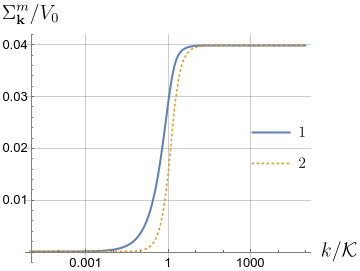
\includegraphics[scale=0.6]{GaussSelfEnergies.png}
\caption{Hartree-Fock self-energies of the Dirac fermions for monolayer and bilayer graphene with the Gaussian potential ($V_{0}=1$ and $a=1$). }
\label{fig:Multilayer-Self-Energies}
\end{figure}

\section{Angular momentum channels and parametrization of the radial coordinate}
In order to exploit the emergent rotational invariance in the thermodynamic limit, we use the following polar parametrization $\mathbf{z}=(k,\phi)$:
\begin{equation}
\label{eq:Tangential-radius}
\begin{split}
    k_{m} &= \frac{\mathcal{K}}{\sqrt{2}} \tan^{2}(n \Delta \theta), 
    \quad \phi_{l}=n\Delta \phi,
\end{split}
\end{equation}
where $(k_n,\phi_l)$ are the polar coordinates of a given site in the polar momentum lattice, $\mathcal{K}$ is the UV momentum scale, $\Delta \theta = (\sfrac{\pi}{2}) /(N+1)$, $\Delta \phi = 2\pi/(2L+1)$, and $l={0,...,2L}$, $n={1,...,N}$. 

Because the Hamiltonian matrix $H_{\mathbf{k k'}}$ that enters into the Hamiltonina $H_{HP}$ in Eq. \eqref{eq:HP-Hamiltonian} of the main text only depends on the difference between the polar angles $\phi-\phi'$ we have conservation of the angular momentum $\ell$ of the bosons. Consequently, we perform Fourier transforms on the polar angle $\phi_{l}$ for the fields $B_{m}^{l\textcolor{white}{\dagger}}$ and the matrix $H_{nn'}^{ll'}$
\begin{equation}
\begin{split}
B_{m}^{l\textcolor{white}{\dagger}} &= 
\frac{1}{\sqrt{2L+1}}\sum_{\ell=-L}^{L}
e^{-i \ell \phi_{l}}B_{m}^{\ell} ,
\\
H_{nn'}^{ll'} &= \sum_{\ell=-L}^{L}
e^{-i \ell (\phi_{l }-\phi_{l'})}
H_{mm'}^{\ell},
\end{split}
\end{equation}
such that the total Bogoliubov Hamiltonian decomposes into a sum of decoupled angular mommentum channels, as follows:
\begin{equation}
H_{HP}^{\textcolor{white}{\ell}} = \sum_{\ell}
H_{HP}^{\ell} = 
\sum_{nn'\ell}
B_{n  }^{\ell\textcolor{black}{\dagger}}
H_{nn'}^{\ell}
B_{n' }^{\ell}.
\end{equation}
Therefore the problem reduces to a set of bosons moving in an effective one dimensional radial space of $N$ sites for each angular momentum channel which in general needs to be solved numerically.	

In that way, each dataset obtained from diagonalizing a $N\times N$ matrix is labelled by the intensity and spreading of the Gaussian potential $V_{0}$ and $a$, respectively, the number of layers $m$, the angular momentum $\ell$ and the number of sites in the radial coordinate $N$.

\section{Bilayer graphene in the channel $\ell=0$}
We begin with the sub-block $\ell = 0$ of the Hamiltonian 
\begin{equation}
H_{HP}^{0} = 
\sum_{mm'0}
B_{m}^{0\textcolor{black}{\dagger}}
H_{mm'}^{0}
B_{m'}^{0}.
\end{equation}
with $V_{0}=1$, $a=1$, $\mathcal{K}=1$ and $m=2$. The self-energy employed to calculate the diagonal elements is shown in \S\ref{sect:Self-Energy}. 

The main result we are interested in is the eigenvalue whose imaginary part is the greatest. We diagonalized $H_{HP}^{0}$ for sizes $N=5$, 10, 20, 50, 100, 200, 500 and 1000, in which we obtained only one complex eigenvalue, whose imaginary part is depicted in the Fig. \ref{fig:MaxImEigVal}. Below $N=5$ there is no imaginary eigenvalue. 

\begin{figure}[h]
\centering
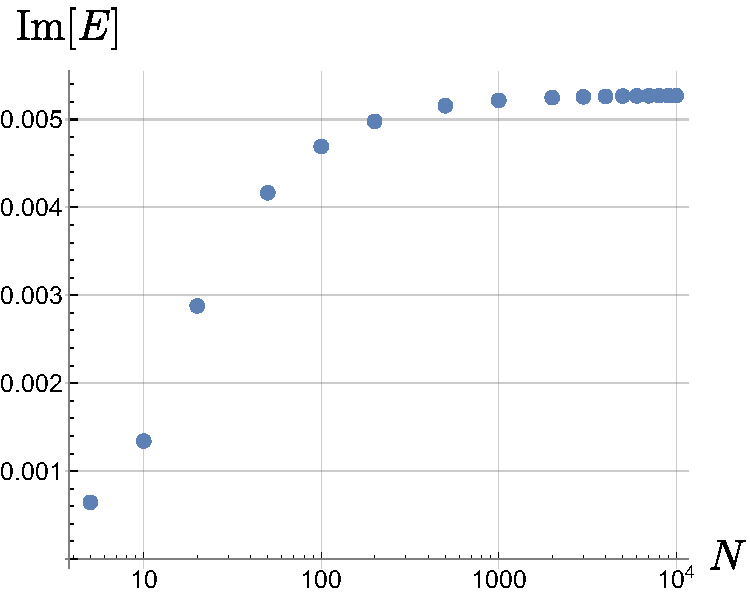
\includegraphics[scale=0.6]{MaxImEigVal.pdf}
\caption{Magnitude of the imaginary part of the only complex eigenvalue vs. number of sites $N$ along radial coordinate $k$.}
\label{fig:MaxImEigVal}
\end{figure}


\begin{comment}
\begin{thebibliography}{10}

\bibitem{giamarchi2003quantum}
T.~Giamarchi, {\em Quantum physics in one dimension}, vol.~121.
\newblock Clarendon press, 2003.

\bibitem{luther1979tomonaga}
A.~Luther, ``Tomonaga fermions and the dirac equation in three dimensions,''
  {\em Physical Review B}, vol.~19, no.~1, p.~320, 1979.

\bibitem{haldane2005luttinger}
F.~Haldane, ``Luttinger's theorem and bosonization of the fermi surface,'' {\em
  arXiv preprint cond-mat/0505529}, 2005.

\bibitem{houghton1993bosonization}
A.~Houghton and J. B. ~Marston, ``Bosonization and fermion liquids in dimensions
  greater than one,'' {\em Physical Review B}, vol.~48, no.~11, p.~7790, 1993.

\bibitem{neto1994bosonization}
A. H. Castro Neto and E.~Fradkin, ``Bosonization of the low energy excitations of
  fermi liquids,'' {\em Physical review letters}, vol.~72, no.~10, p.~1393,
  1994.

\bibitem{houghton2000multidimensional}
A.~Houghton, H.-J. Kwon, and J.~Marston, ``Multidimensional bosonization,''
  {\em Advances in Physics}, vol.~49, no.~2, pp.~141--228, 2000.

\bibitem{neto1995exact}
A. H. Castro Neto and E. H.~Fradkin, ``Exact solution of the landau fixed point via
  bosonization,'' {\em Physical Review B}, vol.~51, no.~7, p.~4084, 1995.

\bibitem{baym1961conservation}
G.~Baym and L.~P. Kadanoff, ``Conservation laws and correlation functions,''
  {\em Physical Review}, vol.~124, no.~2, p.~287, 1961.

\bibitem{PhysRev.127.1391}
G.~Baym, ``Self-consistent approximations in many-body systems,'' {\em Phys.
  Rev.}, vol.~127, pp.~1391--1401, Aug 1962.

\bibitem{PhysRevB.50.7526}
A.~W.~W. Ludwig, M.~P.~A. Fisher, R.~Shankar, and G.~Grinstein, ``Integer
  quantum hall transition: An alternative approach and exact results,'' {\em
  Phys. Rev. B}, vol.~50, pp.~7526--7552, Sep 1994.

\bibitem{ando2002dynamical}
T.~Ando, Y.~Zheng, and H.~Suzuura, ``Dynamical conductivity and zero-mode
  anomaly in honeycomb lattices,'' {\em Journal of the Physical Society of
  Japan}, vol.~71, no.~5, pp.~1318--1324, 2002.

\bibitem{mishchenko2008minimal}
E.~Mishchenko, ``Minimal conductivity in graphene: Interaction corrections and
  ultraviolet anomaly,'' {\em EPL (Europhysics Letters)}, vol.~83, no.~1,
  p.~17005, 2008.

\bibitem{herbut2008coulomb}
I.~F. Herbut, V.~Juri{\v{c}}i{\'c}, and O.~Vafek, ``Coulomb interaction,
  ripples, and the minimal conductivity of graphene,'' {\em Physical review
  letters}, vol.~100, no.~4, p.~046403, 2008.

\bibitem{sheehy2009optical}
D.~E. Sheehy and J.~Schmalian, ``Optical transparency of graphene as determined
  by the fine-structure constant,'' {\em Physical Review B}, vol.~80, no.~19,
  p.~193411, 2009.

\bibitem{abedinpour2011drude}
S.~H. Abedinpour, G.~Vignale, A.~Principi, M.~Polini, W.-K. Tse, and A.~H.
  MacDonald, ``Drude weight, plasmon dispersion, and ac conductivity in doped
  graphene sheets,'' {\em Physical Review B}, vol.~84, no.~4, p.~045429, 2011.

\bibitem{sodemann2012interaction}
I.~Sodemann and M.~M. Fogler, ``Interaction corrections to the polarization
  function of graphene,'' {\em Physical Review B}, vol.~86, no.~11, p.~115408,
  2012.

\bibitem{gazzola2013conductivity}
G.~Gazzola, A.~Cherchiglia, L.~Cabral, M.~Nemes, and M.~Sampaio, ``Conductivity
  of coulomb interacting massless dirac particles in graphene:
  Regularization-dependent parameters and symmetry constraints,'' {\em EPL
  (Europhysics Letters)}, vol.~104, no.~2, p.~27002, 2013.

\bibitem{barnes2014effective}
E.~Barnes, E. H. ~Hwang, R. E. ~Throckmorton, and S. Das Sarma, ``Effective field
  theory, three-loop perturbative expansion, and their experimental
  implications in graphene many-body effects,'' {\em Physical Review B},
  vol.~89, no.~23, p.~235431, 2014.

\bibitem{teber2014interaction}
S.~Teber and A.~Kotikov, ``Interaction corrections to the minimal conductivity
  of graphene via dimensional regularization,'' {\em EPL (Europhysics
  Letters)}, vol.~107, no.~5, p.~57001, 2014.

\bibitem{teber2018field}
S.~Teber and A.~Kotikov, ``Field theoretic renormalization study of interaction
  corrections to the universal ac conductivity of graphene,'' {\em Journal of
  High Energy Physics}, vol.~2018, no.~7, p.~82, 2018.

\bibitem{boyda2016many}
D. L.~Boyda, V. V.~Braguta, M. I.~Katsnelson, and M. V.~Ulybyshev, ``Many-body effects on
  graphene conductivity: Quantum monte carlo calculations,'' {\em Physical
  Review B}, vol.~94, no.~8, p.~085421, 2016.

\bibitem{li2008dirac}
Z.~Li, E.~A. Henriksen, Z.~Jiang, Z.~Hao, M.~C. Martin, P.~Kim, H.~Stormer, and
  D.~N. Basov, ``Dirac charge dynamics in graphene by infrared spectroscopy,''
  {\em Nature Physics}, vol.~4, no.~7, p.~532, 2008.

\bibitem{mak2008measurement}
K.~F. Mak, M.~Y. Sfeir, Y.~Wu, C.~H. Lui, J.~A. Misewich, and T.~F. Heinz,
  ``Measurement of the optical conductivity of graphene,'' {\em Physical review
  letters}, vol.~101, no.~19, p.~196405, 2008.

\bibitem{nair2008fine}
R.~R. Nair, P.~Blake, A.~N. Grigorenko, K.~S. Novoselov, T.~J. Booth,
  T.~Stauber, N.~M. Peres, and A.~K. Geim, ``Fine structure constant defines
  visual transparency of graphene,'' {\em Science}, vol.~320, no.~5881,
  pp.~1308--1308, 2008.

\bibitem{auerbach2012interacting}
A.~Auerbach, {\em Interacting electrons and quantum magnetism}.
\newblock Springer Science \& Business Media, 2012.

\bibitem{SupplementalMaterial}
See the supplemental material for derivations of the expressions.

\bibitem{vanHemmen1980note}
J.~Van~Hemmen, ``A note on the diagonalization of quadratic boson and fermion
  hamiltonians,'' {\em Zeitschrift f{\"u}r Physik B Condensed Matter}, vol.~38,
  no.~3, pp.~271--277, 1980.

\bibitem{armitage2018weyl}
N. P.~Armitage, E. J.~Mele, and A.~Vishwanath, ``Weyl and dirac semimetals in
  three-dimensional solids,'' {\em Reviews of Modern Physics}, vol.~90, no.~1,
  p.~015001, 2018.

\bibitem{bradlyn2016beyond}
B.~Bradlyn, J.~Cano, Z.~Wang, M.~Vergniory, C.~Felser, R.~J. Cava, and B.~A.
  Bernevig, ``Beyond dirac and weyl fermions: Unconventional quasiparticles in
  conventional crystals,'' {\em Science}, vol.~353, no.~6299, p.~aaf5037, 2016.

\end{thebibliography}
\end{comment}

%\bibliography{Manuscript}
%\bibliographystyle{ieeetr}

\end{document} 
